\section{Thu thập dữ liệu giao dịch}
Bộ dữ liệu được sử dụng trong đồ án là tập dữ liệu giao dịch thẻ tín dụng mô phỏng, gồm 30\,058 giao dịch và 23 cột thuộc tính. Dữ liệu được lưu trữ trên Google Sheets và được nạp trực tiếp vào chương trình bằng thư viện \texttt{pandas} \cite{mckinney2010pandas} dưới dạng CSV. Quá trình nạp dữ liệu và làm sạch dữ liệu lần lượt được trình bày trong Hình \ref{fig:code_loading} và Hình \ref{fig:code_cleaning}.

\begin{figure}[H]
    \centering
    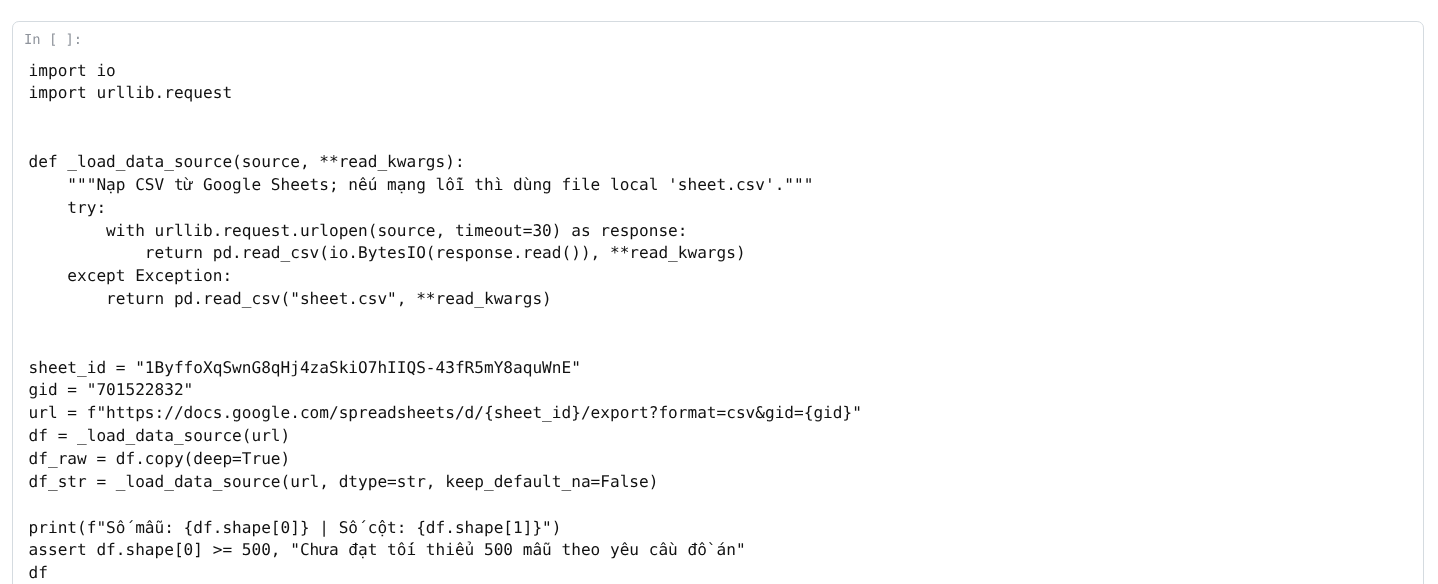
\includegraphics[width=\linewidth,height=0.9\textheight,keepaspectratio]{figures/code_cleaning_1.png}
    \caption{Đoạn chương trình nạp dữ liệu từ Google Sheets}
    \label{fig:code_loading}
\end{figure}

\begin{figure}[htbp]
    \centering
    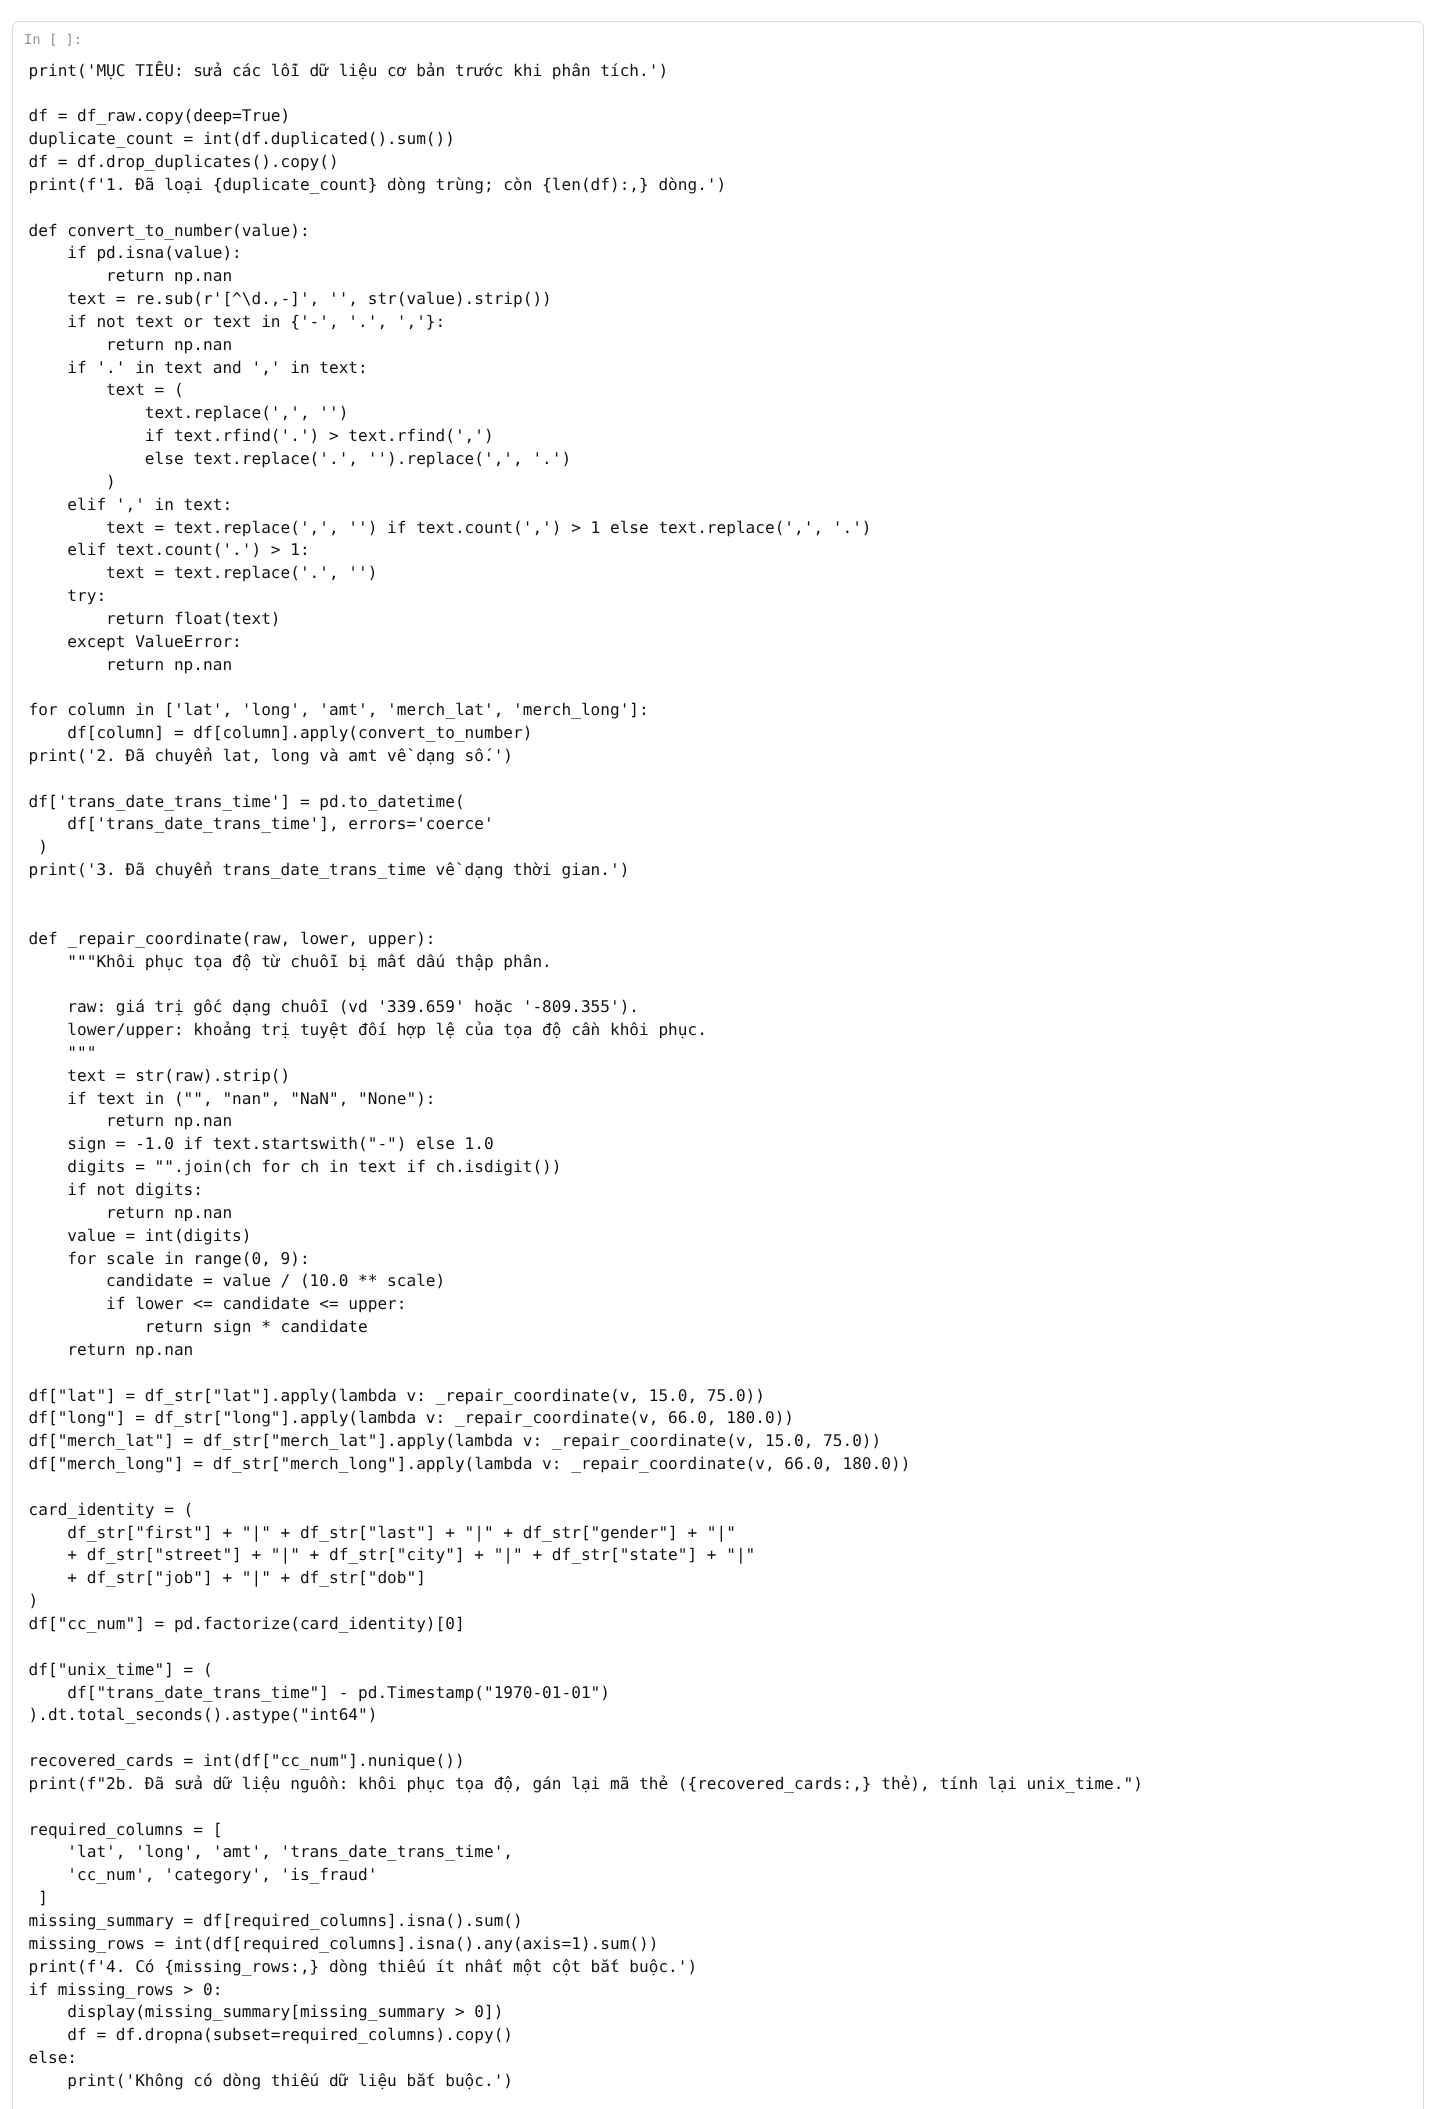
\includegraphics[width=\linewidth,height=0.9\textheight,keepaspectratio]{figures/code_cleaning_2.png}
    \caption{Đoạn chương trình làm sạch dữ liệu}
    \label{fig:code_cleaning}
\end{figure}

\section{Mô tả bộ dữ liệu}
Bộ dữ liệu mô tả hoạt động giao dịch của 909 thẻ tín dụng tại 693 điểm chấp nhận thanh toán thuộc 50 bang của Hoa Kỳ, trong khoảng thời gian 10 ngày, từ ngày 21/06 đến ngày 30/06/2020. Mỗi bản ghi tương ứng với một giao dịch. Số tiền giao dịch dao động từ 1\,USD đến 6\,600{,}44\,USD, với trung vị 46{,}28\,USD. Bảng \ref{tab:data_fields} liệt kê chi tiết các cột quan trọng của bộ dữ liệu.

\begin{table}[H]
\centering
\fontsize{11}{13.6}\selectfont
\renewcommand{\arraystretch}{1.2}
\setlength{\tabcolsep}{6pt}
\begin{tabularx}{\textwidth}{|p{4.2cm}|p{2.2cm}|X|}
\hline
\textbf{Đặc trưng} & \textbf{Kiểu dữ liệu} & \textbf{Mô tả} \\
\hline
trans\_date\_trans\_time & datetime & Thời điểm giao dịch \\
\hline
cc\_num & string & Mã thẻ tín dụng \\
\hline
merchant & string & Đơn vị chấp nhận thanh toán \\
\hline
category & string & Loại hình dịch vụ như mua sắm, ăn uống, du lịch \\
\hline
amt & float & Số tiền giao dịch (USD) \\
\hline
gender & string & Giới tính chủ thẻ \\
\hline
city / state & string & Thành phố / bang nơi giao dịch \\
\hline
lat / long & float & Vĩ độ / kinh độ vị trí thường trú của chủ thẻ \\
\hline
city\_pop & int & Dân số thành phố \\
\hline
job / dob & string & Nghề nghiệp / ngày sinh chủ thẻ \\
\hline
trans\_num / unix\_time & string & Mã giao dịch / thời gian dạng epoch \\
\hline
merch\_lat / merch\_long & float & Vị trí của đơn vị chấp nhận thanh toán \\
\hline
is\_fraud & int & Nhãn: 0 = hợp lệ, 1 = gian lận \\
\hline
\end{tabularx}
\caption{Các đặc trưng của bộ dữ liệu}
\label{tab:data_fields}
\end{table}

Phân bố nhãn của bộ dữ liệu cho thấy tính mất cân bằng nghiêm trọng: có 29\,925 giao dịch hợp lệ nhưng chỉ có 133 giao dịch gian lận, tương ứng tỷ lệ gian lận 0{,}44\%. Lớp lớn gấp 225 lần lớp nhỏ. Vì vậy, Accuracy không phản ánh đúng khả năng phát hiện gian lận của mô hình và không được dùng làm tiêu chí đánh giá chính trong đồ án.

\section{Tiền xử lý dữ liệu}
\subsection{Làm sạch dữ liệu}
Các cột số như \texttt{amt}, \texttt{lat}, \texttt{long}, \texttt{merch\_lat}, \texttt{merch\_long} có thể chứa ký tự hoặc dấu phân cách không mong muốn, được chuẩn hóa về dạng số thực bằng hàm \texttt{convert\_to\_number}. Cột \texttt{trans\_date\_trans\_time} được chuyển sang kiểu \texttt{datetime} để có thể trích xuất giờ giao dịch. Kiểm tra cho thấy bộ dữ liệu không có dòng trùng lặp hoàn toàn và không có dòng thiếu các cột bắt buộc gồm \texttt{lat}, \texttt{long}, \texttt{amt}, \texttt{trans\_date\_trans\_time}, \texttt{cc\_num}, \texttt{category} và \texttt{is\_fraud}; toàn bộ 30\,058 giao dịch được giữ lại cho các bước phân tích tiếp theo.

Quá trình kiểm tra dữ liệu nguồn phát hiện ba lỗi phát sinh khi bộ dữ liệu được nhập vào Google Sheets, được khôi phục trước khi phân tích: (1) các cột tọa độ \texttt{lat}, \texttt{long}, \texttt{merch\_lat}, \texttt{merch\_long} bị mất dấu chấm thập phân (ví dụ \texttt{33{,}9659} bị nhập thành \texttt{339.659}), được khôi phục bằng cách tách toàn bộ chữ số rồi dịch dấu thập phân về bậc sao cho giá trị rơi vào khoảng hợp lệ của vĩ độ (15--75) và kinh độ (66--180); (2) cột mã thẻ \texttt{cc\_num} bị làm tròn về ba chữ số có nghĩa nên chỉ còn 309 mã khác nhau, được thay bằng định danh thẻ ổn định suy ra từ định danh chủ thẻ (họ, tên, địa chỉ, thành phố, bang, nghề nghiệp, ngày sinh), thu được 909 thẻ; (3) cột \texttt{unix\_time} bị ghi đè toàn bộ bằng cùng một hằng số, được tính lại từ cột \texttt{trans\_date\_trans\_time}.

\subsection{Tạo đặc trưng}
Từ dữ liệu thô, một số đặc trưng hành vi được tạo thêm để phục vụ mô hình hóa, minh họa trong Hình \ref{fig:code_features}. Danh sách 14 đặc trưng đầu vào gồm:
\begin{itemize}
    \item \texttt{amt}, \texttt{age}, \texttt{hour}: số tiền giao dịch, tuổi chủ thẻ và giờ trong ngày của giao dịch.
    \item \texttt{amt\_vs\_card\_median}, \texttt{amt\_vs\_card\_avg}: chênh lệch và tỷ lệ giữa số tiền giao dịch với trung vị, trung bình số tiền của thẻ, phản ánh giao dịch lệch thói quen chi tiêu.
    \item \texttt{txn\_freq\_hour}, \texttt{txn\_count\_recent}: tần suất giao dịch của cùng một thẻ trong một giờ và số giao dịch gần đây, phản ánh hoạt động bất thường.
    \item \texttt{distance\_km}, \texttt{speed\_kmh}: khoảng cách từ vị trí của đơn vị chấp nhận thanh toán đến vị trí thường trú của thẻ (tính theo công thức Haversine) và tốc độ di chuyển giữa giao dịch hiện tại với giao dịch trước của cùng thẻ. Vì tọa độ \texttt{lat}/\texttt{long} cố định theo từng thẻ, khoảng cách này phản ánh việc giao dịch ở nơi xa nơi ở quen thuộc.
    \item \texttt{amt\_log}, \texttt{amt\_zscore\_card}: logarit số tiền và mức độ lệch của số tiền so với trung bình thẻ theo độ lệch chuẩn.
    \item \texttt{amt\_per\_km}: tỷ lệ giữa số tiền giao dịch và khoảng cách di chuyển.
    \item \texttt{is\_night}: cờ cho biết giao dịch xảy ra vào ban đêm (từ 22 giờ đến 5 giờ).
    \item \texttt{category}: loại hình dịch vụ.
\end{itemize}

Các đặc trưng thống kê theo thẻ (card profile) chỉ được ước lượng trên tập huấn luyện, còn các đặc trưng phụ thuộc lịch sử riêng của thẻ như \texttt{speed\_kmh}, \texttt{txn\_count\_recent} được tính riêng trong từng tập, nhằm tránh rò rỉ thông tin từ tập kiểm tra vào quá trình huấn luyện.

\begin{figure}[H]
    \centering
    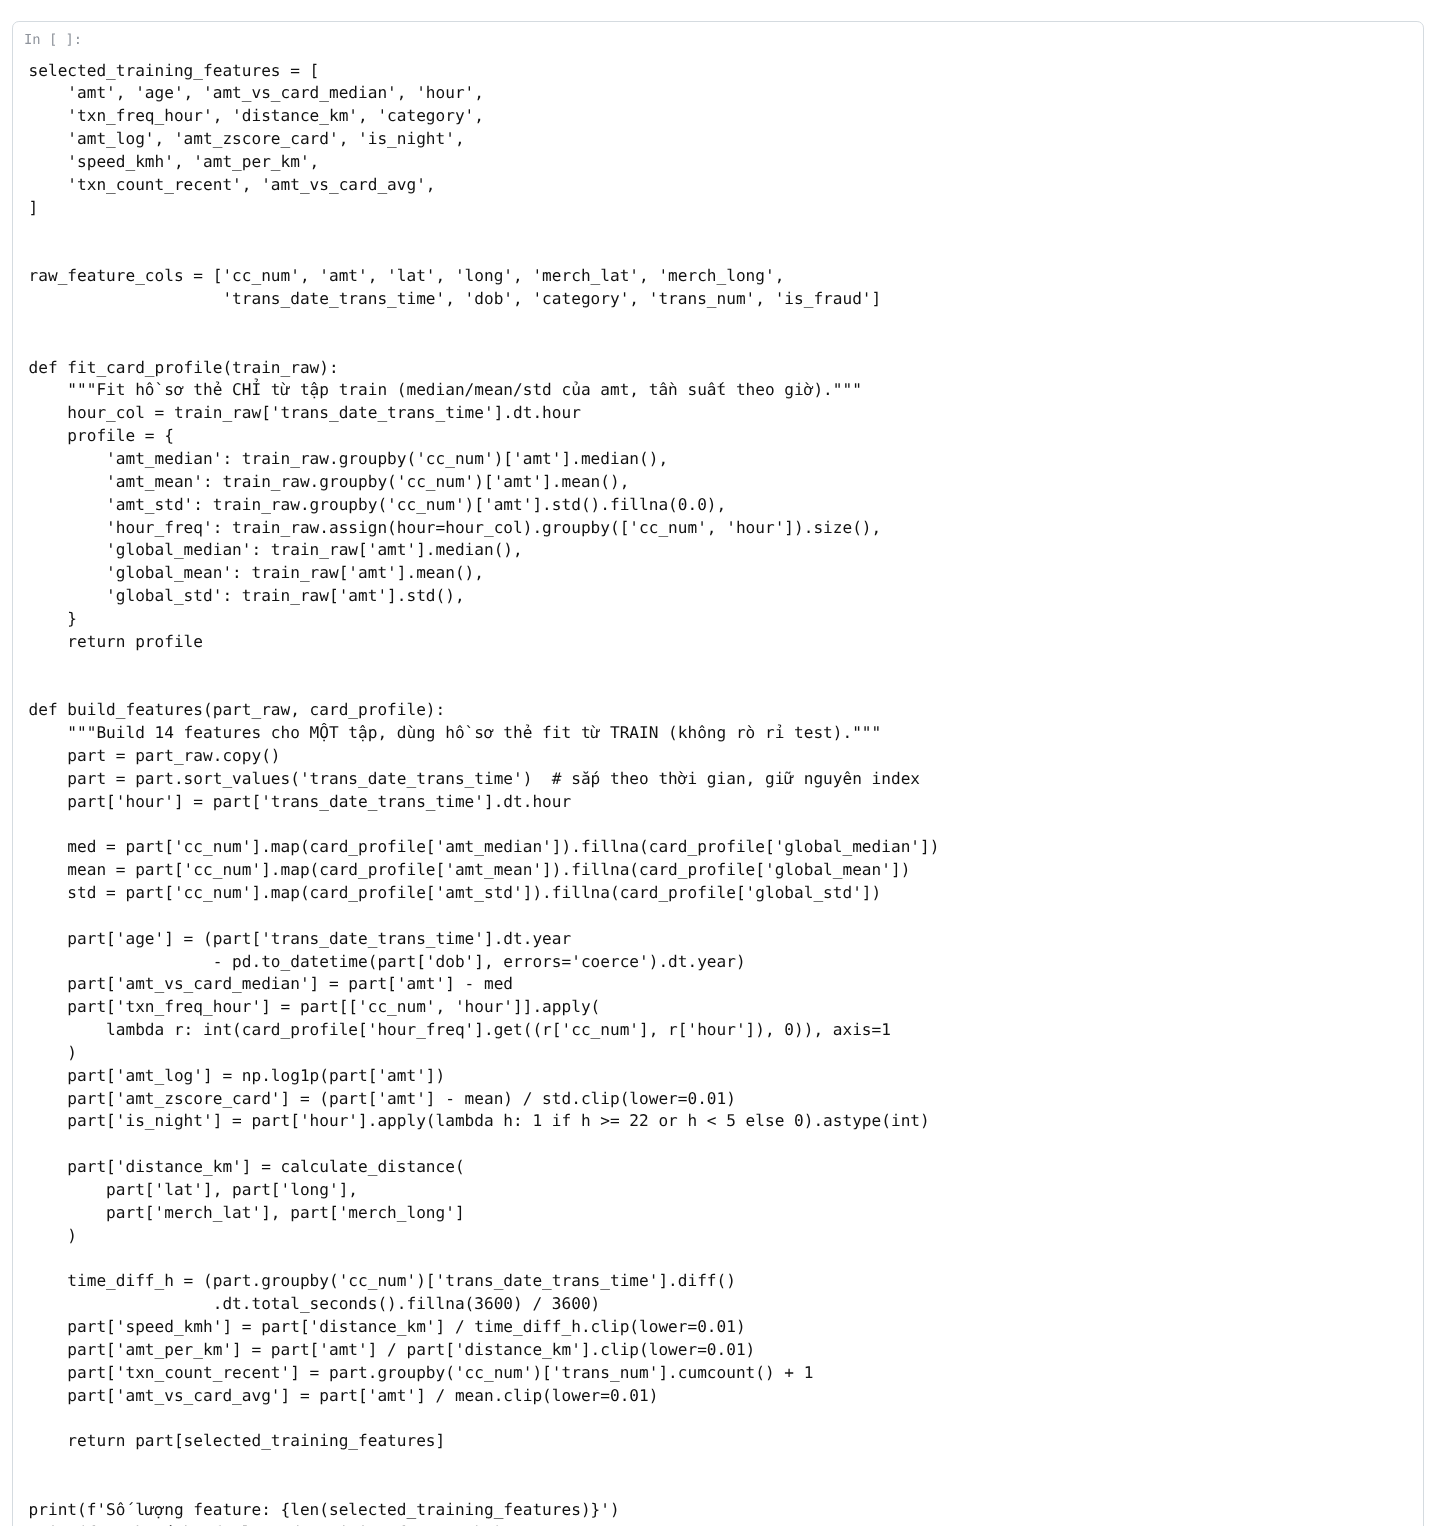
\includegraphics[width=\linewidth,height=0.9\textheight,keepaspectratio]{figures/code_features_1.png}
    \caption{Đoạn chương trình tạo các đặc trưng hành vi}
    \label{fig:code_features}
\end{figure}

Tóm lại, bài toán phân loại giao dịch thẻ tín dụng được phát biểu như sau: đầu vào là một giao dịch được mô tả bằng 14 đặc trưng gồm các giá trị số như số tiền, tuổi, giờ giao dịch, tần suất giao dịch, khoảng cách và tốc độ di chuyển, cũng như loại hình dịch vụ; đầu ra là nhãn phân loại 0 (giao dịch hợp lệ) hoặc 1 (giao dịch gian lận). Mô hình học máy trả về xác suất gian lận của từng giao dịch, sau đó ngưỡng quyết định được sử dụng để chuyển xác suất đó thành nhãn cuối cùng.